% !TEX encoding = UTF-8 Unicode
% TEX template for final reports @ Laboratory of Robotics
% design by Sebastjan Slajpah
% sebastjan.slajpah@fe.uni-lj.si
% May 2023 @ Robolab


\documentclass[a4paper]{article}

\usepackage[utf8]{inputenc}
\usepackage{erk}
\usepackage{times}
\usepackage{graphicx}
\usepackage[top=22.5mm, bottom=22.5mm, left=22.5mm, right=22.5mm]{geometry}

\usepackage[english]{babel}
\usepackage{url}
\usepackage{hvlogos}
\usepackage{array, booktabs}   % for professional tables
\usepackage{amsmath}

% local definitions
\def\footnotemark{}%  to avoid footnote on cover page

\begin{document}
%make title
\title{Instructions and Template for Project's Final Report}

\author{First Author$^{1}$, Mentor$^{2}$} % use ^1, ^2 for author(s) from different institutions

\affiliation{$^{1}$Faculty of Electrical Engineering, University of Ljubljana, Tržaška c. 25, 1000 Ljubljana \\
$^{2}$2Affiliation of mentor’s organisation, if it is not Faculty of Electrical Engineering}

\email{E-mail: author@email.com}

\maketitle


\begin{abstract}{Abstract}
An English abstract is required. The abstract should be no more than 200 words. It should provide a concise summary of the research conducted and highlight what is unique in your work.
\end{abstract}

\section{Introduction}


The final report should be written in the \LaTeX\ environment on an A4 paper with two columns and all outer margins set to 2.25 cm. The report should be four pages in length, including figures, tables, and references. Footnotes and page numbers should be omitted from the report.

For references, use IEEE style \cite{ieee2023}. The bibliography should be included in a separate file (\verb".bib") in \BibTeX\ format. Examples of citing styles can be seen in the References section: book \cite{mihelj2019robotics}, paper \cite{abbott2007pseudo}, and proceedings \cite{beravs2011development}.

\section{Instructions for authors}

Please use the styles defined in this document and do not change the font size or style. You can use this document as a template for writing your report. This template is based on the template for the International Electrotechnical and Computer Science Conference ERK.

The paper should follow the classical structure: Abstract -- Introduction -- Methods -- Results and Discussion -- Conclusion -- References. For more details, please see~\cite{structure2023}.

Each first paragraph should not be indented, but all subsequent paragraphs should have a first line indent.

\subsection{Equations}

Equations and formulas should be written in italics and consecutively numbered. In the text, references to equations should be written in brackets as Eq. \eqref{eq:eq1} -- Eq. \eqref{eq:eq4}.

\begin{equation}
 \int^{r_{2}}_{0}F(r,\varphi)\; dr\; d\varphi= [\sigma r_{2} / (2\mu_{0})]
    \label{eq:eq1}
\end{equation}

\begin{align}
        x &=  v \cdot t     \label{eq:eq2} \\
        v &= a \cdot t      \label{eq:eq3}\\
        a &= \frac{\partial v}{\partial t}      \label{eq:eq4}
\end{align}

\subsection{Tables}

Tables are used to summarize research results. When designing tables, vertical lines should be omitted if they are not necessary. Tables need to be referenced in the text. See Table \ref{tab:table1} for an example.

\begin{table}[htbp]
    \centering
    \caption{Table description with explained abbreviations}
    \label{tab:table1}
    \begin{tabular}{lcccc}
        \toprule
        & \multicolumn{2}{c}{Red} & \multicolumn{2}{c}{White} \\
        \cmidrule(lr){2-3}\cmidrule(lr){4-5}
          & $\Delta t$  & $\bar{x}$    & $\Delta t$  & $\bar{x}$ \\  
        \midrule
        Sub. 1 & $2.3$ & $-0.2$ & $1.7$ & $-1.2$ \\
        Sub. 2 & $2.4$ & $1.2$ & $2.1$ & $3.2$ \\
        sub. 3 & $1.9$ & $2.8$ & $1.8$ & $1.7$  \\
        \bottomrule
    \end{tabular}
\end{table}

\subsection{Figures}

Reports are not printed in colour, so please prepare figures that are appropriate for black-and-white printing. The width of figures should be one or two column widths. Each figure must be labelled with a number and a caption. In the text, each figure must be referenced (Fig. \ref{fig:fig1}).

\begin{figure}[!htb]
    \begin{center}
        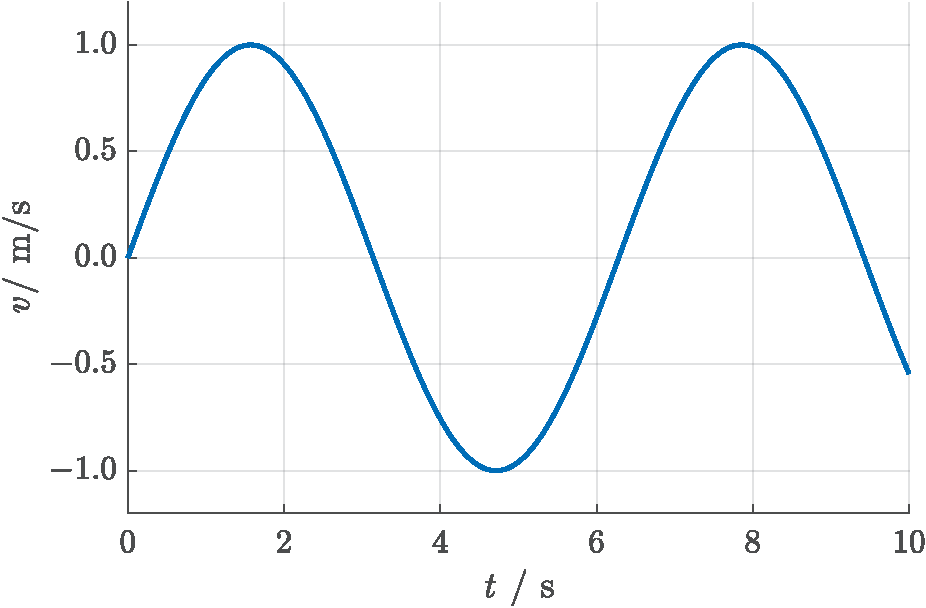
\includegraphics[width=\columnwidth]{signal_fig.pdf}
        \caption{Figure caption describing the content} \label{fig:fig1}
    \end{center}
\end{figure}


Figures must be prepared in a manner that is easy to read, with marked axes and a legend if multiple signals are presented. Figures should be minimalistic, presenting only vital information. Anything that does not add information is a distraction. Figures should be exported in \verb".pdf" format.

\section{Submitting report}

An electronic version of your report in PDF format must be submitted via the student portal at \url{e.fe.uni-lj.si}. The deadline for submission of reports and the time slot for oral presentations will be defined and communicated to you.


\small

\bibliographystyle{ieeetr}
\bibliography{sample_bib}


\end{document}